\documentclass[aspectratio=169,11pt]{beamer}

\usetheme{Madrid}
\usecolortheme{seagull}
\setbeamertemplate{navigation symbols}{}

\usepackage{amsmath,amssymb}
\usepackage{booktabs}
\usepackage{graphicx}
\usepackage{hyperref}

\graphicspath{{../../results/figures/}{assets/}}

\definecolor{CSSBlue}{RGB}{16,52,96}
\definecolor{CSSAccent}{RGB}{5,117,107}
\setbeamercolor{title}{fg=CSSBlue}
\setbeamercolor{frametitle}{fg=CSSBlue}
\setbeamercolor{structure}{fg=CSSAccent}

\title{Counterfactual Structural Sensitivity (CSS)}
\subtitle{Dataset-Only Probing under Minimal Linguistic Edits}
\author[V. Rathore \& S. Aneesh]{Vidhi Rathore (2023121002) \and Sambu Aneesh (2023121012)}
\institute{Computational Psycholinguistics Project}
\date{Spring 2026}

\begin{document}

\begin{frame}
  \titlepage
\end{frame}

\begin{frame}{Presentation Roadmap}
\begin{enumerate}
  \item Problem framing
  \item CSS protocol and math
  \item Datasets, models, and setup
  \item Results and completion status
  \item Remaining work and finalization plan
\end{enumerate}
\end{frame}

\begin{frame}{Problem Framing}
\begin{itemize}
  \item Minimal edits can flip sentence meaning (role swap, negation insertion/removal).
  \item We test whether hidden-state geometry reacts to these edits in a structured way.
  \item Current project track is strictly dataset-only and does not use human annotation.
\end{itemize}
\begin{block}{Core Question}
Do representation-shift metrics and probe signals systematically track counterfactual structural edits?
\end{block}
\end{frame}

\begin{frame}{CSS Protocol}
\small
\[
\text{sentence } s
\rightarrow
\text{counterfactual } s_{cf}
\rightarrow
\text{hidden states}
\rightarrow
\Delta\text{-metrics}
\]
\[
\rightarrow
\text{probes}
\rightarrow
\text{GPT-2 surprisal}
\rightarrow
\text{dataset-level statistical summary}
\]
\normalsize
\vspace{0.4em}
\begin{itemize}
  \item Representation extraction at embedding + layers \(1\ldots 12\).
  \item One row per pair, model, layer, and metric.
\end{itemize}
\end{frame}

\begin{frame}{Dataset Scope (GitHub-Only)}
\begin{table}
\centering
\begin{tabular}{lcc}
\toprule
\textbf{Module} & \textbf{Pairs} & \textbf{Source} \\
\midrule
Role reversal & 1500 & Extending Psycholinguistic Dataset \\
Negation & 1500 & Extending Psycholinguistic Dataset \\
\midrule
\textbf{Total} & \textbf{3000} & GitHub dataset only \\
\bottomrule
\end{tabular}
\end{table}
\begin{itemize}
  \item Active merged file: \texttt{full\_all\_3000.jsonl}.
  \item Attachment and human-annotation tracks are excluded from this run.
\end{itemize}
\end{frame}

\begin{frame}{Models and Representations}
\begin{itemize}
  \item Models:
  \texttt{bert-base-uncased}, \texttt{roberta-base}, \texttt{gpt2}.
  \item Primary representation units:
  \begin{itemize}
    \item mean-pooled sentence vectors,
    \item token matrices with subword-to-word pooling.
  \end{itemize}
  \item Secondary ablations:
  CLS (BERT/RoBERTa), last-token (GPT-2).
\end{itemize}
\end{frame}

\begin{frame}{Primary Metrics}
\small
\[
\Delta_{\cos}^{(l)} = 1 - \cos\!\big(\mu_l(s),\mu_l(s_{cf})\big)
\]
\[
\text{sim}_{\text{frob}}^{(l)} =
\frac{\lVert K(\widehat{A}_l,\widehat{B}_l)\rVert_F}
{\sqrt{\lVert K(\widehat{A}_l,\widehat{A}_l)\rVert_F\lVert K(\widehat{B}_l,\widehat{B}_l)\rVert_F + \varepsilon}}
\]
\[
\Delta_{\text{frob}}^{(l)} = 1 - \text{sim}_{\text{frob}}^{(l)},
\quad
\Delta_{L2}^{(l)} = \lVert \mu_l(s)-\mu_l(s_{cf}) \rVert_2
\]
\[
\Delta_{\text{token}}^{(l)} =
\frac{1}{|M|}\sum_{(i,j)\in M}\left(1-\cos\!\big(h^{(l)}_{i},h^{(l)}_{j,cf}\big)\right)
\]
\end{frame}

\begin{frame}{Probes and Surprisal}
\begin{itemize}
  \item Linear probes by layer:
  role (\(agent/patient\)) and negation (\(0/1\)).
  \item Selectivity controls:
  random-label control, reported as task minus control.
  \item GPT-2 autoregressive surprisal:
  \[
  \text{surprisal}(t_i) = -\log P(t_i \mid t_{<i})
  \]
  \item Reported features:
  total/average surprisal and counterfactual deltas.
\end{itemize}
\end{frame}

\begin{frame}{Dataset-Only Statistical Targets}
\begin{itemize}
  \item D1: per-layer correlation of each CSS metric with
  \( |\Delta \text{avg surprisal}| \).
  \item D2: incremental value of \(\Delta_{\text{frob}}\) over \(\Delta_{\cos}\)
  for surprisal-target regression.
  \item D3: phenomenon/model-specific layer profile differences.
  \item D4: probe selectivity stability across layers.
\end{itemize}
\end{frame}

\begin{frame}{Execution Coverage}
\begin{table}
\centering
\begin{tabular}{lc}
\toprule
\textbf{Component} & \textbf{Status} \\
\midrule
Data import + schema validation & \(\checkmark\) complete \\
Hidden-state extraction (3 models) & \(\checkmark\) complete \\
Metrics (all layers) & \(\checkmark\) complete \\
Probes + selectivity controls & \(\checkmark\) complete \\
GPT-2 surprisal & \(\checkmark\) complete \\
Dataset-only stats (D1--D4) & \(\checkmark\) complete \\
Salience extension + plots & \(\checkmark\) complete \\
\bottomrule
\end{tabular}
\end{table}
\end{frame}

\begin{frame}{Layer Correlation Curves}
\centering
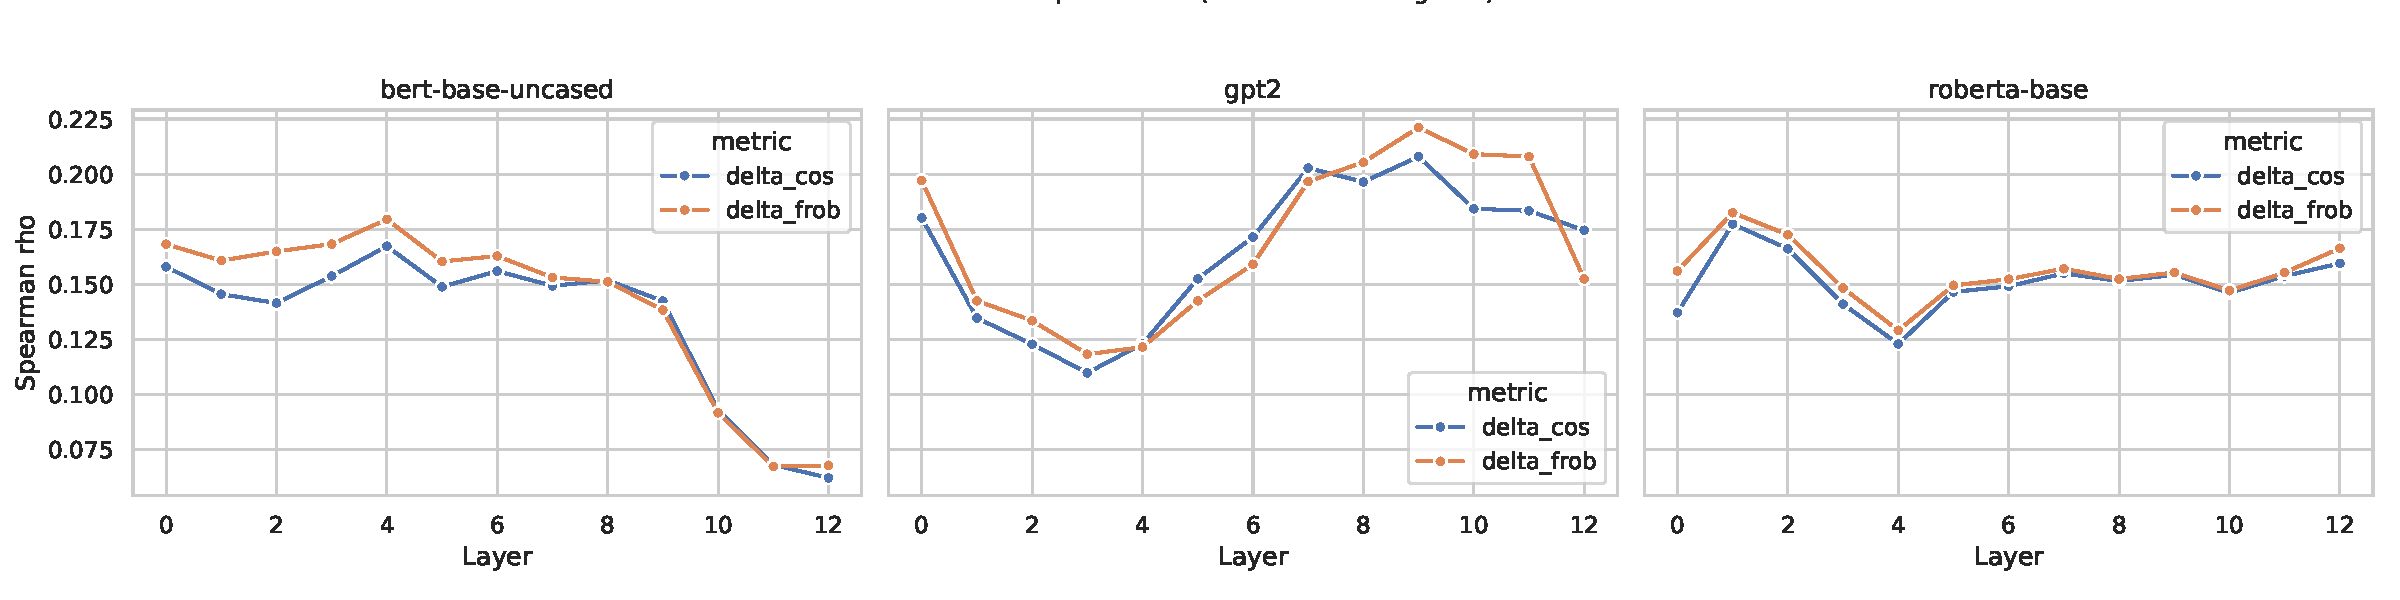
\includegraphics[width=0.92\linewidth]{layer_correlation_curves.pdf}
\vspace{0.4em}

\small Spearman correlation of representation shifts with surprisal deltas.
\end{frame}

\begin{frame}{Probe Selectivity Curves}
\centering
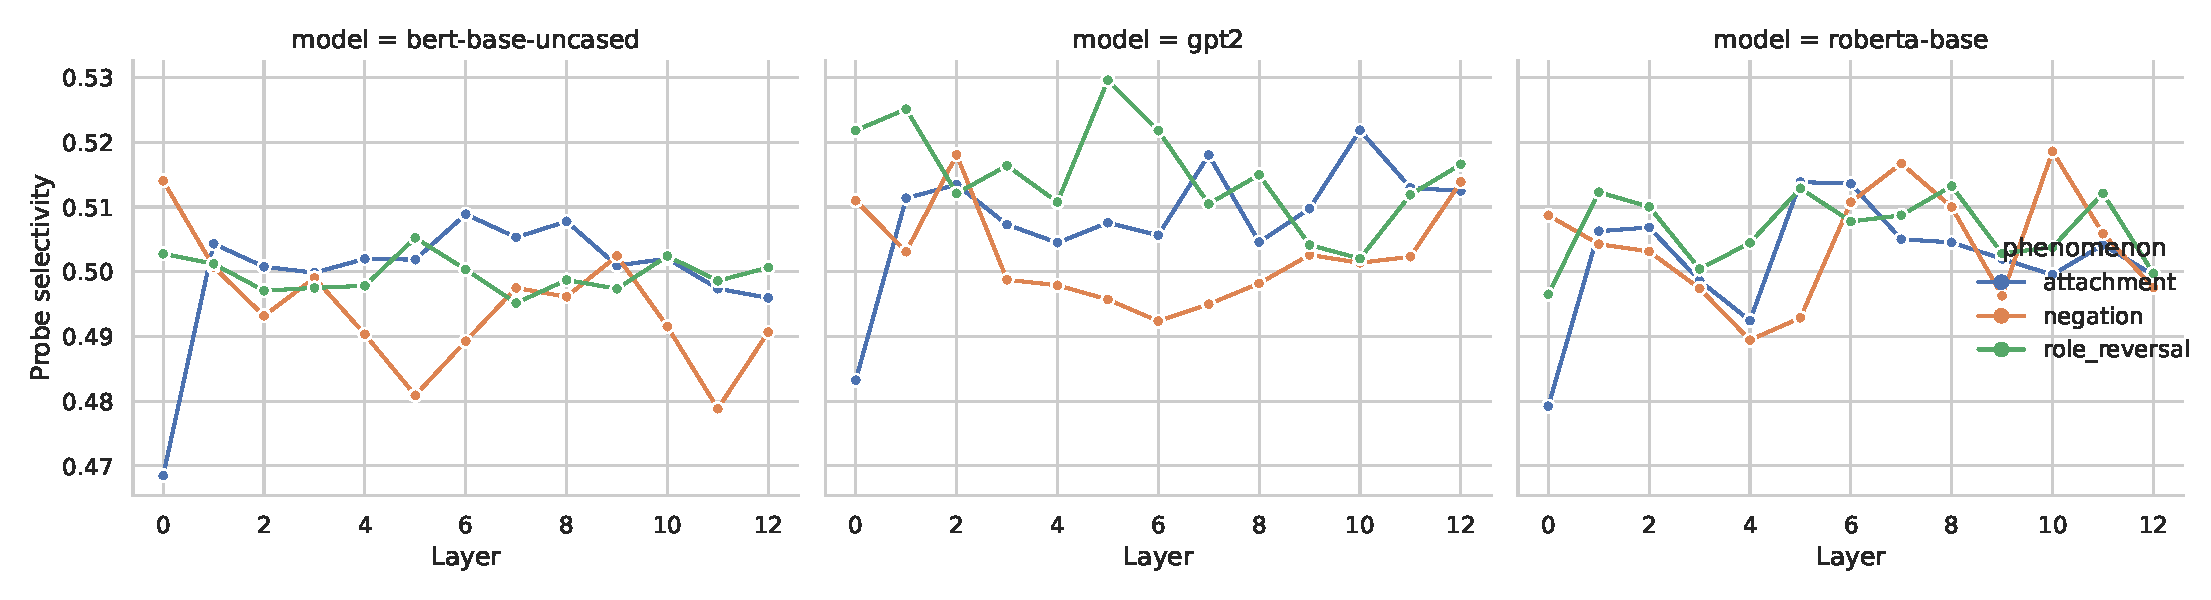
\includegraphics[width=0.92\linewidth]{probe_selectivity_curves.pdf}
\vspace{0.4em}

\small Selectivity \(=\) task macro-F1 minus random-label macro-F1.
\end{frame}

\begin{frame}{Frobenius Shift vs Surprisal Delta}
\centering
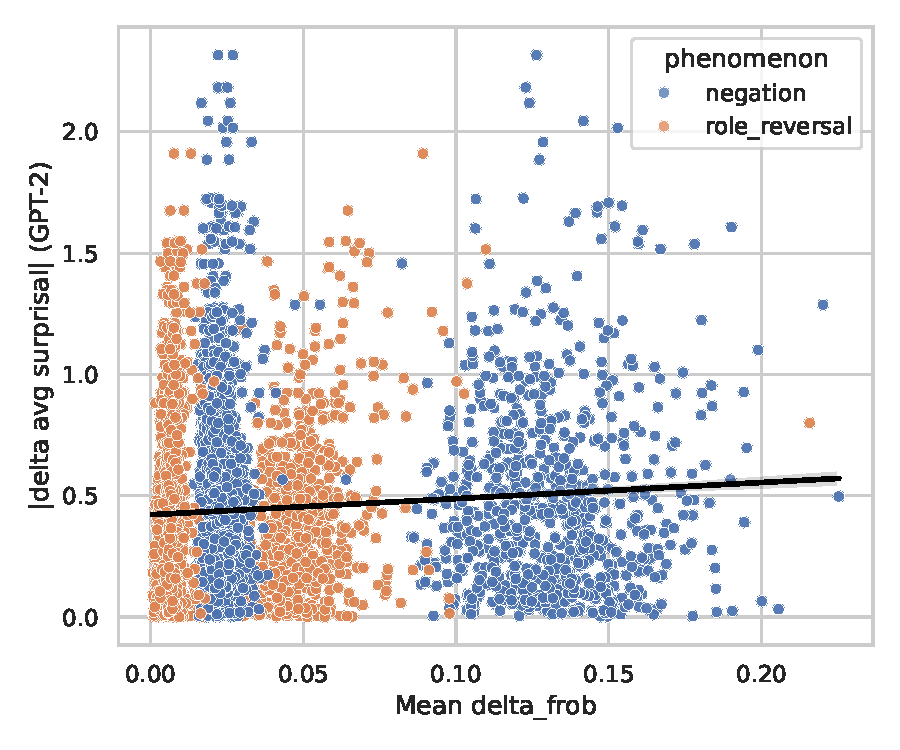
\includegraphics[width=0.88\linewidth]{surprisal_vs_shift.pdf}
\vspace{0.4em}

\small Pair-level aggregation over models/phenomena: \(\Delta_{\text{frob}}\) vs \( |\Delta \text{avg surprisal}| \).
\end{frame}

\begin{frame}{Current Interpretation}
\begin{itemize}
  \item Pipeline is fully executable and reproducible with modern toolchain (\texttt{uv}, config-driven scripts, cached artifacts).
  \item Frobenius, cosine, token-aligned, and L2 metrics are all available per layer and per model.
  \item Final claims are strictly dataset-only structural sensitivity claims.
\end{itemize}
\end{frame}

\begin{frame}{What Is Left}
\begin{enumerate}
  \item Final write-up polish for dataset-only claim language.
  \item Final table curation for D1--D4 summary.
  \item Submission packaging and presentation rehearsal.
\end{enumerate}
\end{frame}

\begin{frame}{Final Timeline}
\begin{table}
\centering
\begin{tabular}{ll}
\toprule
\textbf{Week} & \textbf{Milestone} \\
\midrule
Week 1 & Final tables/plots lock and narrative freeze \\
Week 2 & Paper text polish and appendix cleanup \\
Week 3 & Final presentation rehearsal and submission \\
\bottomrule
\end{tabular}
\end{table}
\end{frame}

\begin{frame}{Conclusion}
\begin{itemize}
  \item CSS pipeline is complete on role + negation GitHub data.
  \item Full model set (BERT, RoBERTa, GPT-2) and full metric set are executed.
  \item Remaining work is packaging and final communication, not core computation.
\end{itemize}
\vspace{0.6em}
\centering
\Large Thank you.
\end{frame}

\begin{frame}{References (Core)}
\footnotesize
\begin{itemize}
  \item Devlin et al. (2019), BERT.
  \item Liu et al. (2019), RoBERTa.
  \item Radford et al. (2019), GPT-2.
  \item Warstadt et al. (2020), BLiMP.
  \item Hewitt and Liang (2019), probe controls.
  \item Levy (2008), surprisal.
  \item vor der Bruck and Pouly (2019), matrix norms for similarity.
\end{itemize}
\end{frame}

\end{document}
